\chapter{Far Detector}
\label{ch:annex-rate}

\section{Overview}

A number of parameters from DUNE/LBNF requirements, design documents,  and studies are used  as input
for estimations of the data rates in DUNE. In cases when derived parameters need to be generated based on these inputs
this is accomplished using the software package \textit{dune-params}\cite{duneparams}
developed specifically for this purpose.
As the inputs and estimations are refined the results presented in
this annex can be regenerated at will.

Because the triggering and readout strategy and algorithms of the DAQ and
analyses are under development and far from their final state of readiness,
the data rate estimations involve some broad assumptions and leave open some choices.
This is described in more detail in the following subsections.



\section{Thresholds for the LArTPC Data Rate Estimations}

There are three threshold levels considered for the purposes of characterizing the LArTPC data rates.
These thresholds are assumed to be applied ``per-wire'' and on the basis of ADC values (which can be translated
to units like MeV with proper calibration).
Optimizing these thresholds for physics require additional study and
are used here only to provide benchmarks for the data rate estimations.
The data produced at each threshold are termed:

\begin{description}
\item[full-stream] The full-stream (FS) threshold means there is no threshold at all.
FS data is data where every time bin (as defined by the ADC clock) on every channel is read out.
\item[zero-suppressed] The zero-suppression (ZS) threshold is an ADC
  level roughly corresponding to what an \chargezsthreshold deposition
  would produce in a single time bin on a single wire.
  All bins with ADC counts below this threshold are remove from the
  data stream.
\item[high-energy] A high-energy (HE) threshold is assumed which is
  such that all signals from radioactive decays are suppressed but low
  enough to not impact activity from beam neutrino interactions or
  potential nucleon decay activity.
  Further studies are needed to determine this threshold but currently
  it is taken, without rigor, to be \SI{1}{\MeV}--\SI{10}{MeV}.
\end{description}

\section{Assumption on the DAQ}

The data rate estimates make the following assumptions on the DAQ capabilities.
In discussion with the DAQ experts they are expected to be satisfied.
More information on the DAQ is available in the Volume 4 of the CDR.

\begin{itemize}
\item The DAQ trigger farm will be able to identify isolated activity
  collected in a single APA consistent with $^{39}Ar$ decay in order
  to suppress reading it to the DAQ data farm.
\item The RCEs will be able to apply a zero suppression
  algorithms with a given threshold to data sent to the trigger farm.
\item The RCEs will be able to apply trigger-specific zero suppression
  algorithms and thresholds to the data sent to the data farm.
\item RCE-local data storage is left open as a possibility.
\end{itemize}

\section{Sources of Data in the TPC}

The data rate estimates are produced considering a specific sources of
data.

\begin{description}
\item[in-spill] Any activity in the detector which is coincident with
  the passage of beam neutrinos through the detector.
\item[with-beam-$\nu$] A subset of \textit{in-spill} where activity is
  consistent with a beam-$\nu$ interacting in the detector.
\item[cosmic-$\mu$] Activity due to the passing of cosmic-ray muons
  through the detector.
\item[radioactivity] Activity due to the decay of radioactive
  isotopes.
\item[atm-$\nu$] Activity consistent with interactions from
  atmospheric neutrinos.
\item[noise] Fluctuation in electronics noise (common-mode not considered).
\end{description}

\section{Fundamental Parameters of the LArTPC}

This section provides a selection of fundamental parameters used as
input to the data rate estimations.
The parameters are summarized in
table~\ref{tab:fundamental-parameters}

% do not edit, this is generated by dune-params
\begin{tabular}[h]{l|r}
\hline
Full height & \SI[round-mode=places,round-precision=1]{12.0}{\meter} \\
Full width & \SI[round-mode=places,round-precision=1]{14.5}{\meter} \\
Full length & \SI[round-mode=places,round-precision=1]{58.0}{\meter} \\
Detectors & \num[round-mode=places,round-precision=0]{4.0} \\
\hline
channel/APA & \num[round-mode=places,round-precision=0]{2560.0} \\
APA/detector & \num[round-mode=places,round-precision=0]{150.0} \\
Active height (APA) & \SI[round-mode=places,round-precision=1]{6.0}{\meter} \\
Active width (APA) & \SI[round-mode=places,round-precision=1]{2.3}{\meter} \\
Drift distance & \SI[round-mode=places,round-precision=2]{3.6}{\meter} \\
\hline
Drift velocity & \SI[round-mode=places,round-precision=1]{1.6}{\milli\meter\per\micro\second} \\
Drift time & \SI[round-mode=places,round-precision=0]{2.25}{\milli\second} \\
\hline
bytes/sample & \SI[round-mode=places,round-precision=1]{1.5}{\byte} \\
sample rate & \SI[round-mode=places,round-precision=1]{2.0}{\mega\hertz} \\
\# drifts/readout & \num[round-mode=places,round-precision=1]{2.4} \\
\hline
readout time & \SI[round-mode=places,round-precision=0]{5.4}{\milli\second} \\
samples/readout & \num[round-mode=places,round-precision=0]{10800.0} \\
\hline
\end{tabular}

\section{Full-stream Data}

Full-stream (FS) data corresponds to reading all data in every ADC channel without application of any threshold.
Estimating its rate is an exact calculation based on known parameters as it does not depend on
the activity in the detector or the noise level of the electronics.
As its name implies, it is the most voluminous type of data that can be generated by the TPC.
The parameters which apply to this data are given in table~\ref{tab:full-stream-parameters}.

% do not edit, this is generated by dune-params

\begin{cdrtable}[Full-stream data rate parameters.]{lr}{tab:full-stream-parameters}{Parameters pertaining to full-stream data rates.}
Parameter & Value \\ \toprowrule

Bytes per sample & \SI[round-mode=places,round-precision=1]{1.5}{\byte} \\ \colhline

DAQ sample rate & \SI[round-mode=places,round-precision=1]{2.0}{\mega\hertz} \\ \colhline

Channels per APA & \num[round-mode=places,round-precision=0]{2560.0} \\ \colhline

Number of APA per detector module & \num[round-mode=places,round-precision=0]{150.0} \\ \colhline

Number of modules & \num[round-mode=places,round-precision=0]{4.0} \\ \colhline

Total channels in DUNE & \num[round-mode=places,round-precision=0]{1536000.0} \\ \colhline

Drifts per readout & \num[round-mode=places,round-precision=1]{2.4} \\ \colhline

Drift time & \SI[round-mode=places,round-precision=2]{2.25}{\milli\second} \\ \colhline

Beam spill repetition rate & \SI[round-mode=places,round-precision=2]{0.833333333333}{\hertz} \\ \colhline

Annual run time fraction & \num[round-mode=places,round-precision=3]{0.667} \\ \colhline

\end{cdrtable}

The expected data rates for two scenarios of FS data are given
in table~\ref{tab:full-stream-volume}.
The first row gives the data size of one DAQ readout (\daqreadouttime).
The second is appropriate for any strategy that intends to record FS
data for each beam spill.
The third contains two numbers that characterize data volume relevant to a strategy which aims to record FS data
for Supernova Burst candidates.
The final row  shows the total annual data volume that the DUNE DAQ is capable of producing (in theory).
These numbers are not meant to imply ongoing recording of full-stream
data to permanent storage.

% do not edit, this is generated by dune-params
\begin{tabular}[h]{l|r}
\hline
Full-stream readout size & \SI[round-mode=places,round-precision=1]{24.8832}{\giga\byte} \\
\hline
Full-stream in-spill data rate & \SI[round-mode=places,round-precision=0]{436.461066147}{\peta\byte\per\year} \\
\hline
Full-stream 1 second data volume & \SI[round-mode=places,round-precision=1]{4.608}{\tera\byte} \\
Full-stream 1 minute data volume & \SI[round-mode=places,round-precision=1]{276.48}{\tera\byte} \\
\hline
Full-stream 1 year data volume & \SI[round-mode=places,round-precision=1]{145.414314891}{\exa\byte} \\
\hline
\end{tabular}

\section{Zero-suppressed Data}

There are options in choosing the exact zero-suppression (ZS) procedure,
and the final choice has not been made.
For these data rate estimates a very simple procedure is assumed: in each
channel, all digitized time bins in which the ADC values are below
the given threshold are removed.
More discussion on possible alternative ZS methods and their impact on
the data rate are give below.

The nominal ZS threshold is assumed to be the ADC counts produced when
the equivalent of \chargezsthreshold energy is deposited and the
ionized wire is collected by a single wire.
It is assumed that the application of zero-suppression at this
threshold completely removes ADC counts due to just noise although an
estimate of data rates due to noise is given.

Estimations of different sources of ZS data are summarized in table~\ref{tab:zs-volume}.

% do not edit, this is generated by dune-params
% per 40kt DUNE
% name, event rate, event size, data rate, annual data volume
\begin{cdrtable}[Zero-suppressed data rates.]{rrrrr}{zs-volume}{Data rate estimations for ZS data from various sources. An additional FS data estimation is given for supernova burst (SNB).}
Source & Event Rate & Event Size & Data Rate & Annual Data Volume \\ \toprowrule
\colhline
all $^{39}Ar$ & \SI[round-mode=places,round-precision=1]{11.16}{\mega\hertz} & \SI[round-mode=places,round-precision=0]{150.0}{\byte} & \SI[round-mode=places,round-precision=1]{1.674}{\giga\byte\per\second} &  \SI[round-mode=places,round-precision=0]{52.8262940816}{\peta\byte}\\
all in-spill & & & & \SI[round-mode=places,round-precision=0]{158.558121686}{\tera\byte} \\
with-beam-$\nu$ & & & & \SI[round-mode=places,round-precision=0]{79.279060843}{\giga\byte} \\
\colhline
cosmic-$\mu$ & \SI[round-mode=places,round-precision=3]{0.258947264}{\hertz} &
\SI[round-mode=places,round-precision=1]{2.5}{\mega\byte} & \SI[round-mode=places,round-precision=1]{647.36816}{\kilo\byte\per\second} &
\SI[round-mode=places,round-precision=0]{20.4289491035}{\tera\byte} \\
\colhline
beam-$\nu$ & \SI[round-mode=places,round-precision=0]{8770.19567714}{\per\year} & \SI[round-mode=places,round-precision=1]{2.5}{\mega\byte} &
\SI[round-mode=places,round-precision=2]{0.694791666667}{\kilo\byte\per\second} & \SI[round-mode=places,round-precision=0]{21.9254891928}{\giga\byte} \\
\colhline
SNB cand. (ZS) & \SI[round-mode=places,round-precision=0]{12.0}{\per\year} & \SI[round-mode=places,round-precision=1]{16.74}{\giga\byte} &
\SI[round-mode=places,round-precision=0]{6365.63904105}{\byte\per\second} & \SI[round-mode=places,round-precision=0]{200.88}{\giga\byte} \\
SNB cand. (FS) & \SI[round-mode=places,round-precision=0]{12.0}{\per\year} & \SI[round-mode=places,round-precision=1]{46.08}{\tera\byte} &
\SI[round-mode=places,round-precision=1]{17.5226192958}{\mega\byte\per\second} & \SI[round-mode=places,round-precision=0]{552.96}{\tera\byte} \\
\end{cdrtable}

\subsubsection{$^{39}Ar$ Decays}

The $^{39}Ar$ decay could potentially dominate the data volume.
The end point of the $^{39}Ar$ decay is at \SI{565}{\keV} and about
25\% of the beta spectrum is above the ZS threshold\cite{docdb3018}.
The expected total decay rate is
\SI{1.0}{\hertz\per\kilo\gram}\cite{bkds}.

The $^{39}Ar$ ionization is very localized and it is assumed that any
dispersion will not spread the charge out to any extent larger than a
wire pitch nor the distance the charge will drift over one sample.
Based on the expected shaping time that the electronics imposes on the
signal the resulting waveform will be spread over
\SI{10}{\micro\second} or \num{20} samples.
Because offline signal processing is sensitive to tails of waveforms,
even more time samples may be required.
Finally, it is assumed a single collection wire and two induction
wires in each view will register an appreciable signal.

As small as these events are, they are numerous enough that their data
volume is not justified given their relative lack of physics importance.
Some mitigation is required and will be developed.

The simplest mitigation is to increase the ZS threshold to be above
the decay endpoint.
This will produce a negative impact in removing small energy
depositions associated with larger events and thus will only be
considered if absolutely required to mitigate the rate.

A better approach is the one that drives the requirement on the DAQ
that the trigger farm be capable of identifying isolated activity
consistent with $^{39}Ar$ on a per-APA basis in order to veto its
recording.
The DAQ is expected to be able to provide this functionality.
This then leaves $^{39}Ar$ which is accidentally coincident in the
same APA with readouts from other activity such as beam-$\nu$
interaction and cosmic muons.
The annual number of above ZS-threshold $^{39}Ar$ decay events
coincident anywhere in the DUNE detector with beam-$\nu$ activity is
given in table~{ref:zs-volume} as \betainbeamyear.
Of that only 3\% are coincident in the same APA bringing the added
data rate to about 10\% that of the beam-$\nu$ activity.

\subsubsection{Supernova Burst}

The Supernova Burst (SNB) data is estimated assuming a
\textit{false-positive} SNB rate of \snbcandrate and a readout time of
\snbreadouttime.
It should be emphasized that both these parameters are subject to
modification and are used simply to provide benchmark examples.

On possible source of false positive SNB triggers may be an upward
fluctuation in the rate of $^{39}Ar$ decays.
Whatever initiates, it is assumed that the data volume of a
false-positive SNB trigger is dominated by $^{39}Ar$ decays.

In the case of an actual SNB, its neutrino interactions will produce
on order of 1000 events across the far detector modules over a time
around ten seconds and with a neutrino spectrum up to \SI{100}{\MeV}.
Given the importance of collecting SNB neutrinos, the same
trigger-based reduction of $^{39}Ar$ will not be employed and thus it
will dominate the data volume.
These addition data volume due to the SNB events themselves is not
significant.

Further, a lower ZS threshold may be considered for saving such
candidate SNB occurrences.
The possible data rate of SNB candidates is thus bound by the nominal
ZS $^{39}Ar$ rate and the FS rate.
The exact strategy for saving SNB candidates requires additional study
and may have implications on DAQ hardware.

\subsection{Noise}

% fixme: is this remotely true?
The nominal ZS threshold of \chargezsthreshold is based on an older
requirement of a 9:1 signal to noise ratio for a 1 MIP.
The most likely MIP is \SI{1.8}{\MeV/\cm} or \SI{0.9}{\MeV} per wire pitch.
This implies an RMS noise requirement equivalent to \SI{0.1}{\MeV} and
then the \SI{0.5}{\MeV} equivalent ZS threshold represents a $5\sigma$ cut.
Across the \dunenumberchannels channels and the
\daqreadoutchannelsamples per readout gives about \num{5000} samples
above the nominal ZS threshold.
Their distributed nature and isolated appearance make them subject to
the same rejection criteria as isolated $^{39}Ar$ and thus can be
ignored for the purposes of data volume estimates.


\section{High-energy Threshold}

For the purpose of these estimates the  high-energy (HE) threshold is chosen at the level above 
the energy scale of the radiological backgrounds relevant for the LArTPC, and set at  \chargehethreshold.
A more careful study is needed to determine a potentially more optimal value for this threshold.
The data rates with the HE threshold applied are summarized in table~\ref{tab:he-volume}.

% do not edit, this is generated by dune-params
% per 40kt DUNE
% name, event rate, event size, data rate, annual data volume
\begin{tabular}[h]{r|r|r|r|r}
\hline
source & event rate & event size & data rate & annual data volume \\
\hline
$^{39}Ar$ & - & - & - & -\\
\hline
cosmic-$\mu$ & \SI[round-mode=places,round-precision=3]{0.258947264}{\hertz} &
\SI[round-mode=places,round-precision=1]{50.0}{\kilo\byte} & \SI[round-mode=places,round-precision=1]{12.9473632}{\kilo\byte\per\second} &
\SI[round-mode=places,round-precision=0]{408.57898207}{\giga\byte} \\
\hline
beam-$\nu$ & \SI[round-mode=places,round-precision=0]{8770.19567714}{\per\year} & \SI[round-mode=places,round-precision=1]{10.0}{\mega\byte} &
\SI[round-mode=places,round-precision=2]{2.77916666667}{\kilo\byte\per\second} & \SI[round-mode=places,round-precision=0]{87.7019567714}{\giga\byte} \\
\hline
SNB cand. & - & - & - & -\\
\hline
\end{tabular}

With the HE threshold in place, activity from the $^{39}$Ar events and any SNB
candidates will not be visible (i.e. will be rejected in DAQ).
Although actual SNB events may result in neutrino with energies as high as
\SI{100}{\MeV} applying such a high threshold to SNB candidates won't be optimal and is not being considered at this point.
For this reason, contribution from SNB to these data is not calculated for this threshold setting.


\section{Compression}

The above estimates assume that the only compression employed is the
lossy removal of data below some threshold.
In addition, a lossless compression is possible.
The DAQ can employ Huffman encoding during readout or the compression
features provided by ROOT may be provided during file writing.
In order to estimate the effects of compression, specific particle
types and energies were simulated using LArSoft.
The initial kinematics for the simulated samples covered a matrix of
particles ($e$, $\mu$, $\tau$, $\pi^+$, $\pi^-$, $\pi^0$ and proton) and momenta
(\SI{100}{\MeV} to \SI{6}{\GeV}).
The uncompressed and compressed sizes are summarized in figure~\ref{fig:data-compression}.

\begin{cdrfigure}[Event size estimations.]{data-compression}{Estimation of DUNE zero-suppressed event sizes for
    different particles and momenta before (left) and after (center)
    compression and their ratios (right).
    Each line represents one particle type.
    The samples were generated with LArSoft assuming
    \SI{10}{\kilo\tonne} detector module with \num{300000} channels.}

  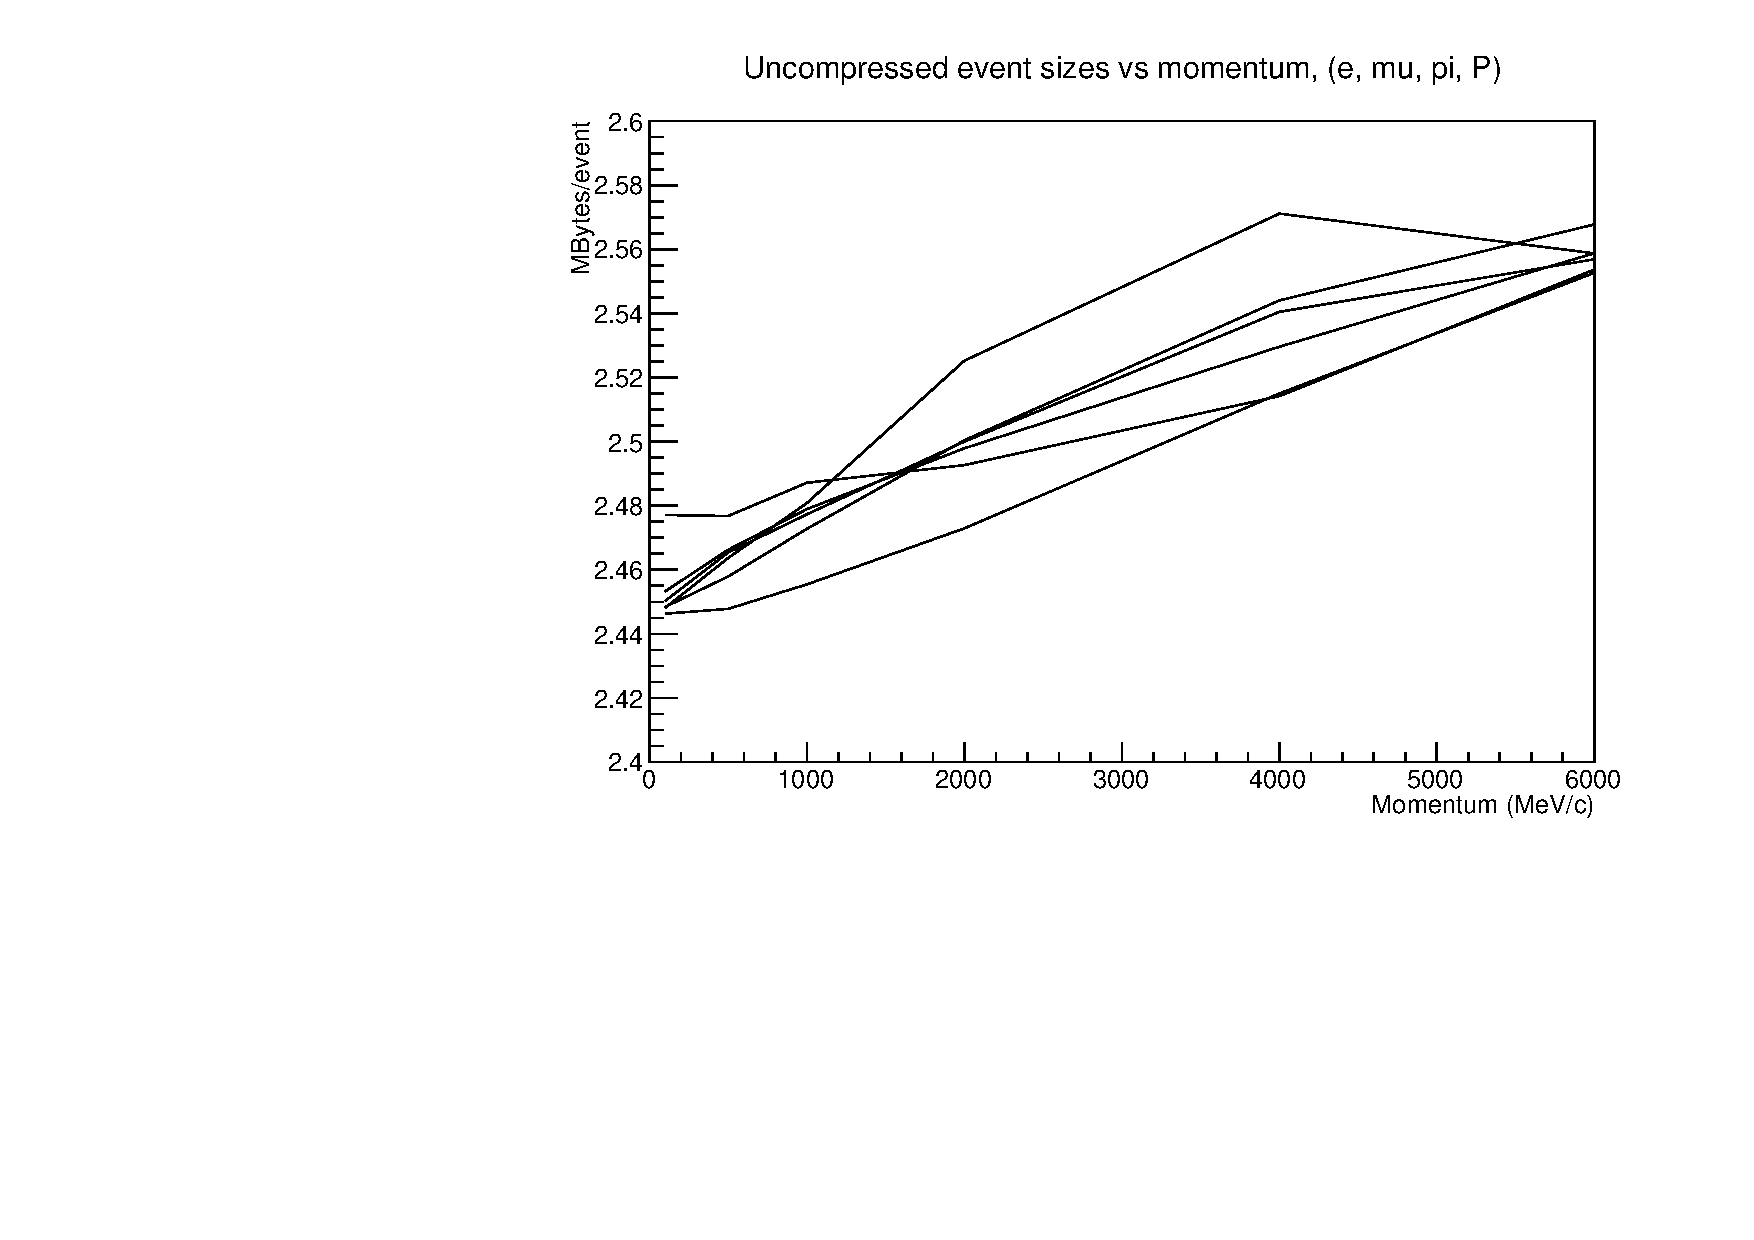
\includegraphics[width=0.3\textwidth]{btot.pdf}
  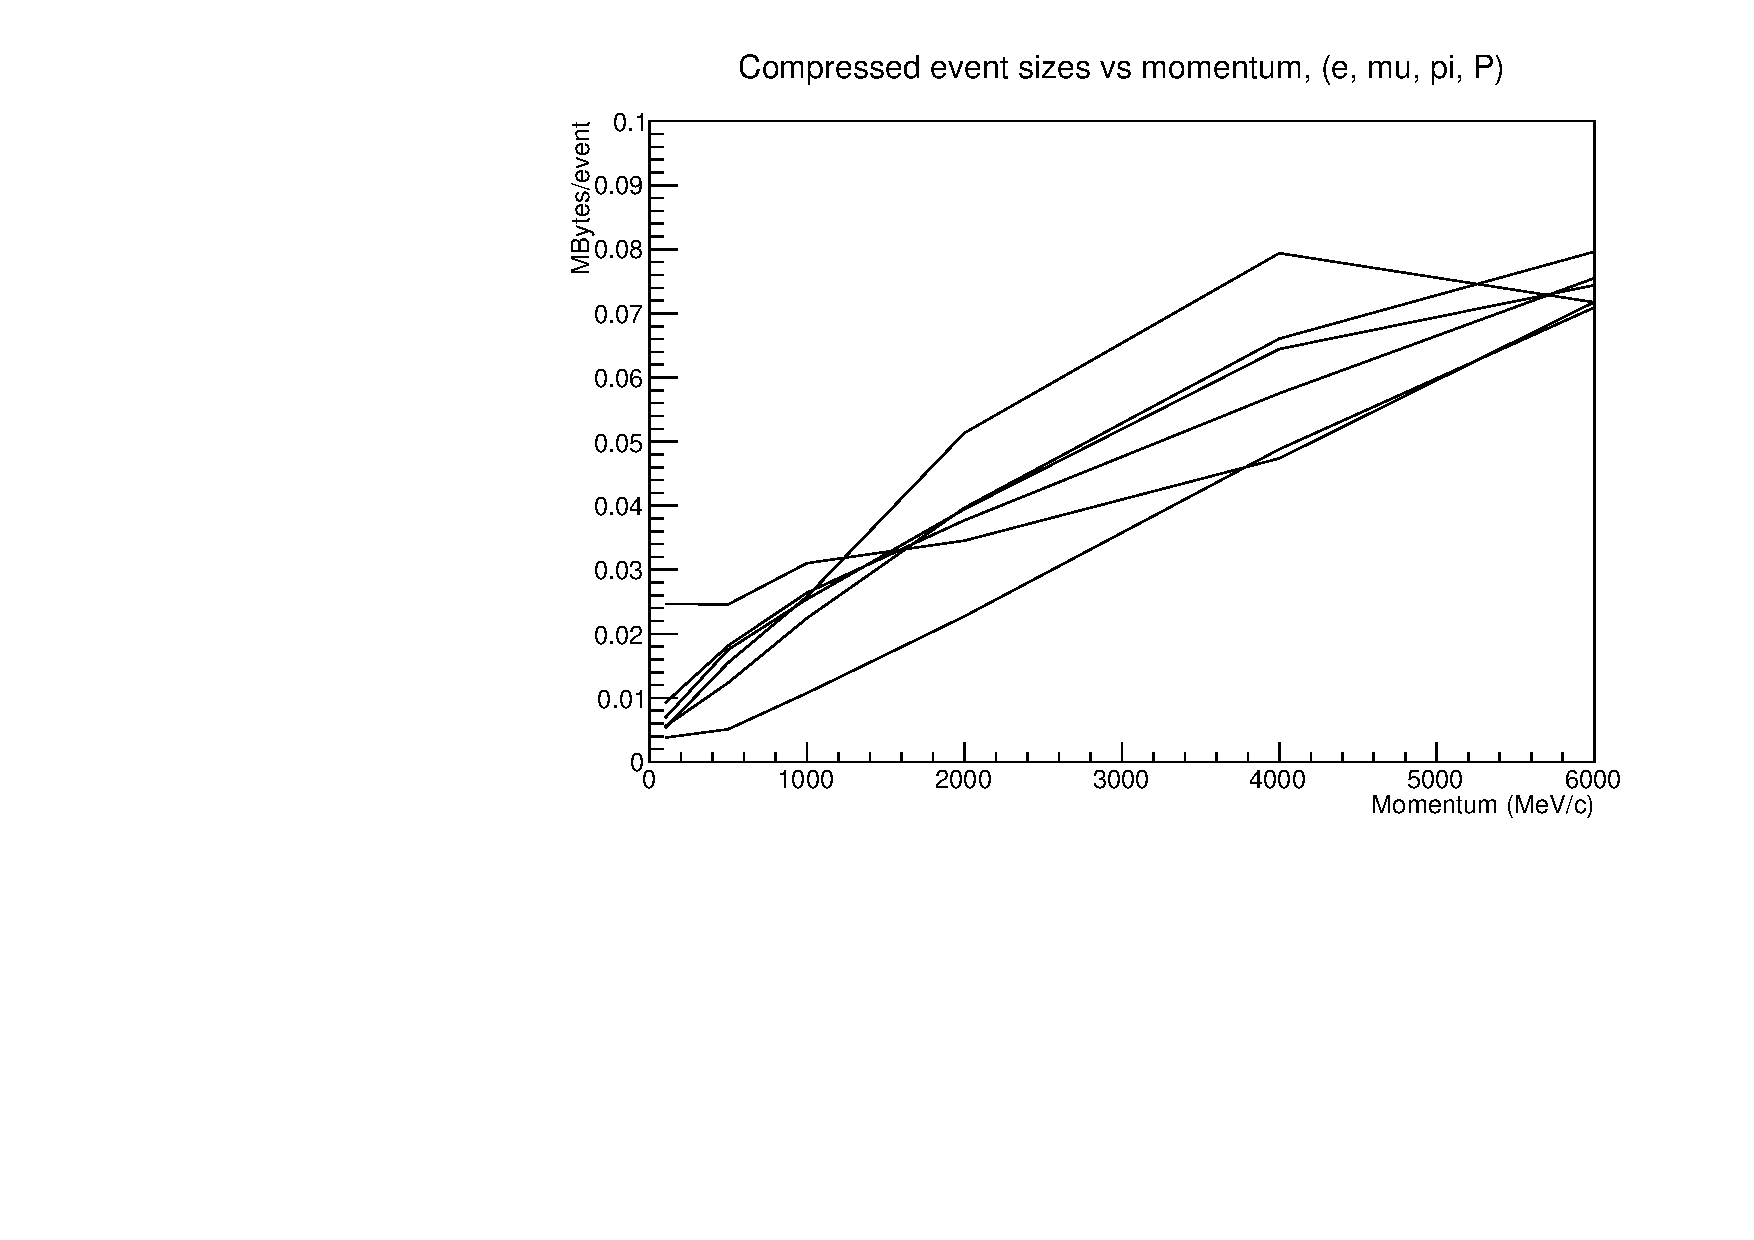
\includegraphics[width=0.3\textwidth]{bzip.pdf}
  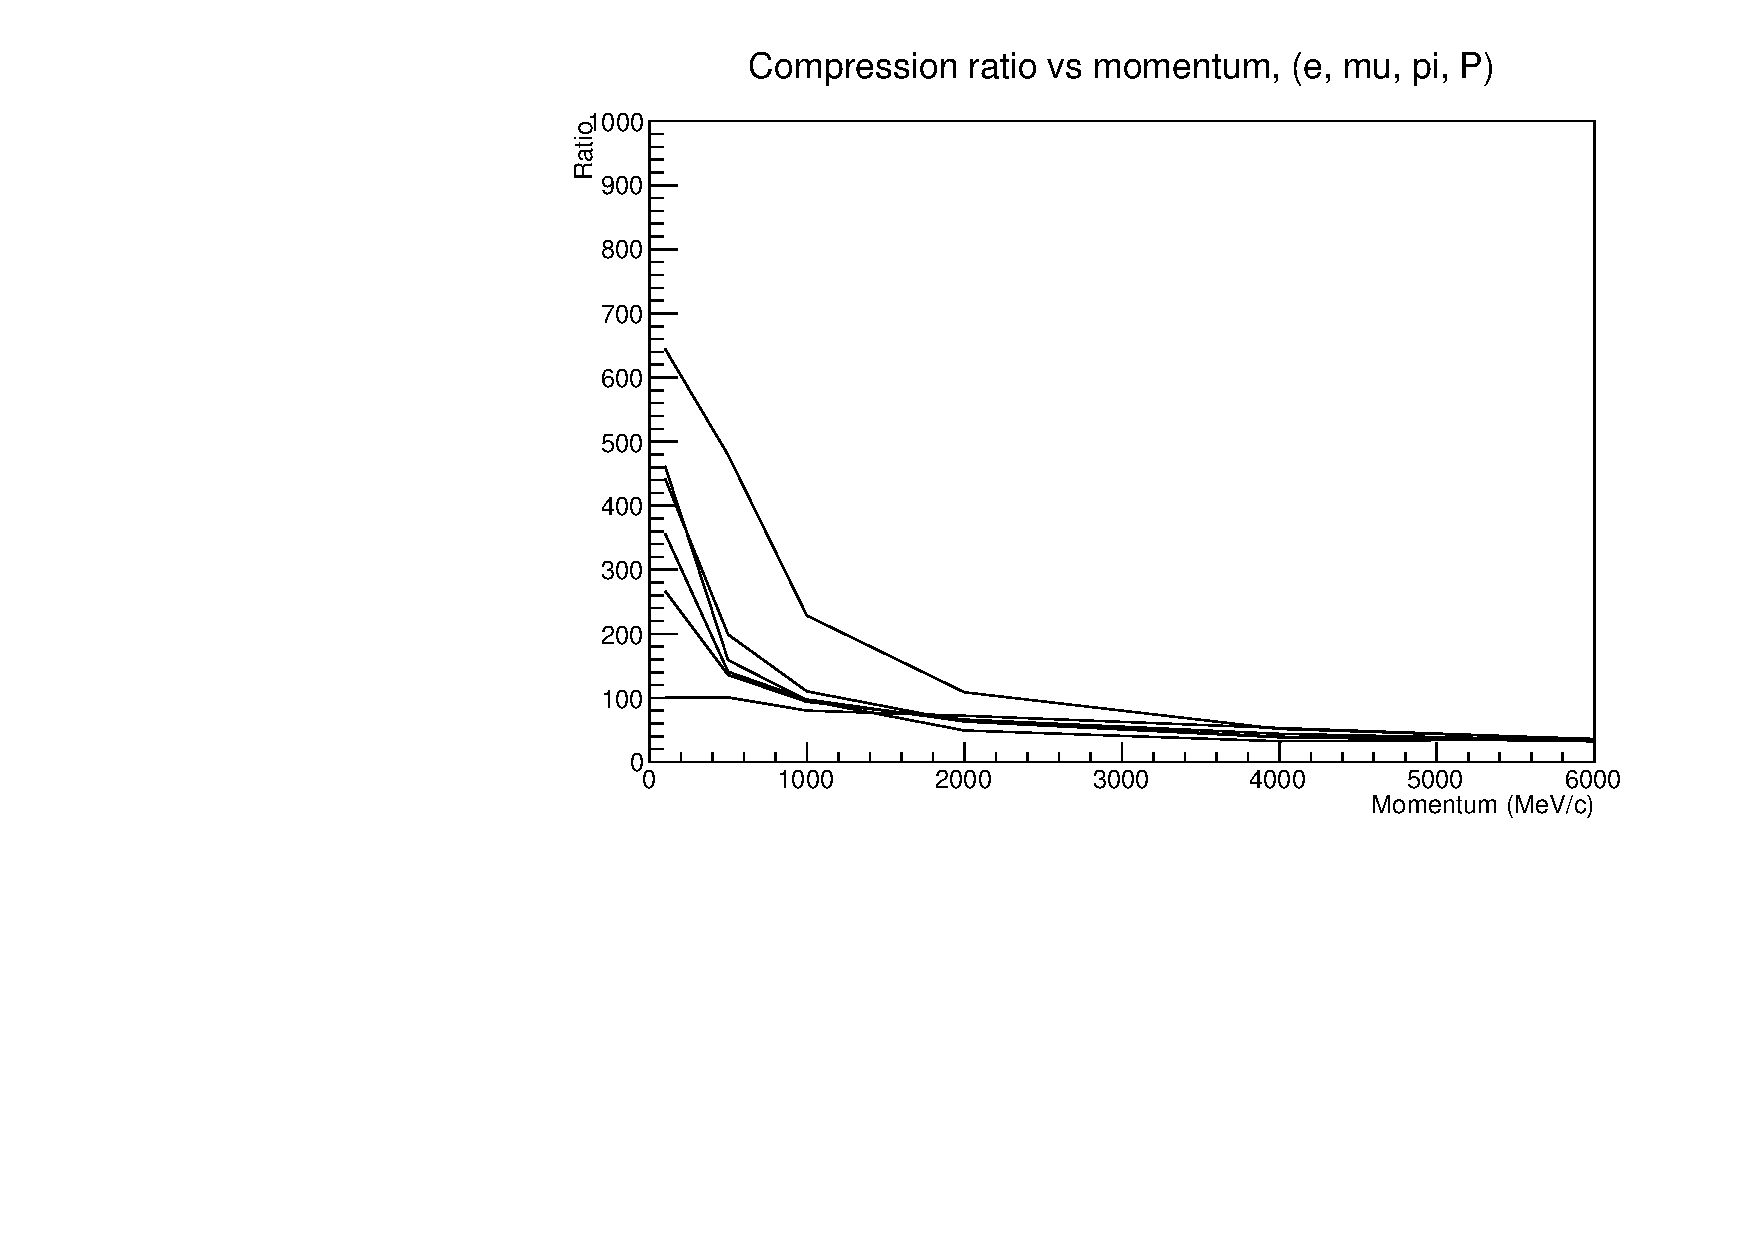
\includegraphics[width=0.3\textwidth]{brat.pdf}

\end{cdrfigure}

It must be noted that this exercise discovered the bulk of the
compressed data written by LArSoft is actually made up channel ID
numbers providing a data inflation of about a factor of 10.
For uncompressed data this added about 50\%.
There are also additional data elements related in the ``raw data''
branch which are superfluous or at best repeated more frequently than
is likely to be required.
In the LArSoft output, even though zero suppression is applied, every
channel has an associated a pedestal and a sigma as well as a
compression number.
There is also a sample count in addition to the one in the sample
vector which is stored.
These values do no vary yet each take up about the same (uncompressed)
size as the ADC values and are significant in size even after
compression.
They are not included in figure~\ref{fig:data-compression}.

Finally, as can be seen in the figure, the change in uncompressed
event size is only a minor function of event momenta and particle types.
It is believed that LArSoft is saving additional overhead for all
channels, even those that have been fully zero-suppressed.

The simulation used a detector module consisting of \num{300000} wires and
thus naively the event size in the full reference detector would be some 5 times
larger.
However, given the arguments above, it is expected that this leads to
a gross over-estimate, possibly by one or two orders of magnitude from
what should be expected if even just a little effort is put into
designing a better storage schema.
Once compression is assumed, the problems with this sub-optimal
storage schema are lessened.
We then select the uncompressed event size to be \beameventsize and
the compressed event size of \beameventsizecompressed based
on~\ref{fig:data-compression}.
We identify this with being the zero-suppressed data produced by just
activity due to beam interactions or similar energy events and accept
the large over-estimation as a generous safety factor.






